\documentclass[./../main_file.tex]{subfiles}
\begin{document}
	\subsection{Mô hình tiến trình}
	\begin{figure}[H]
		\centering
		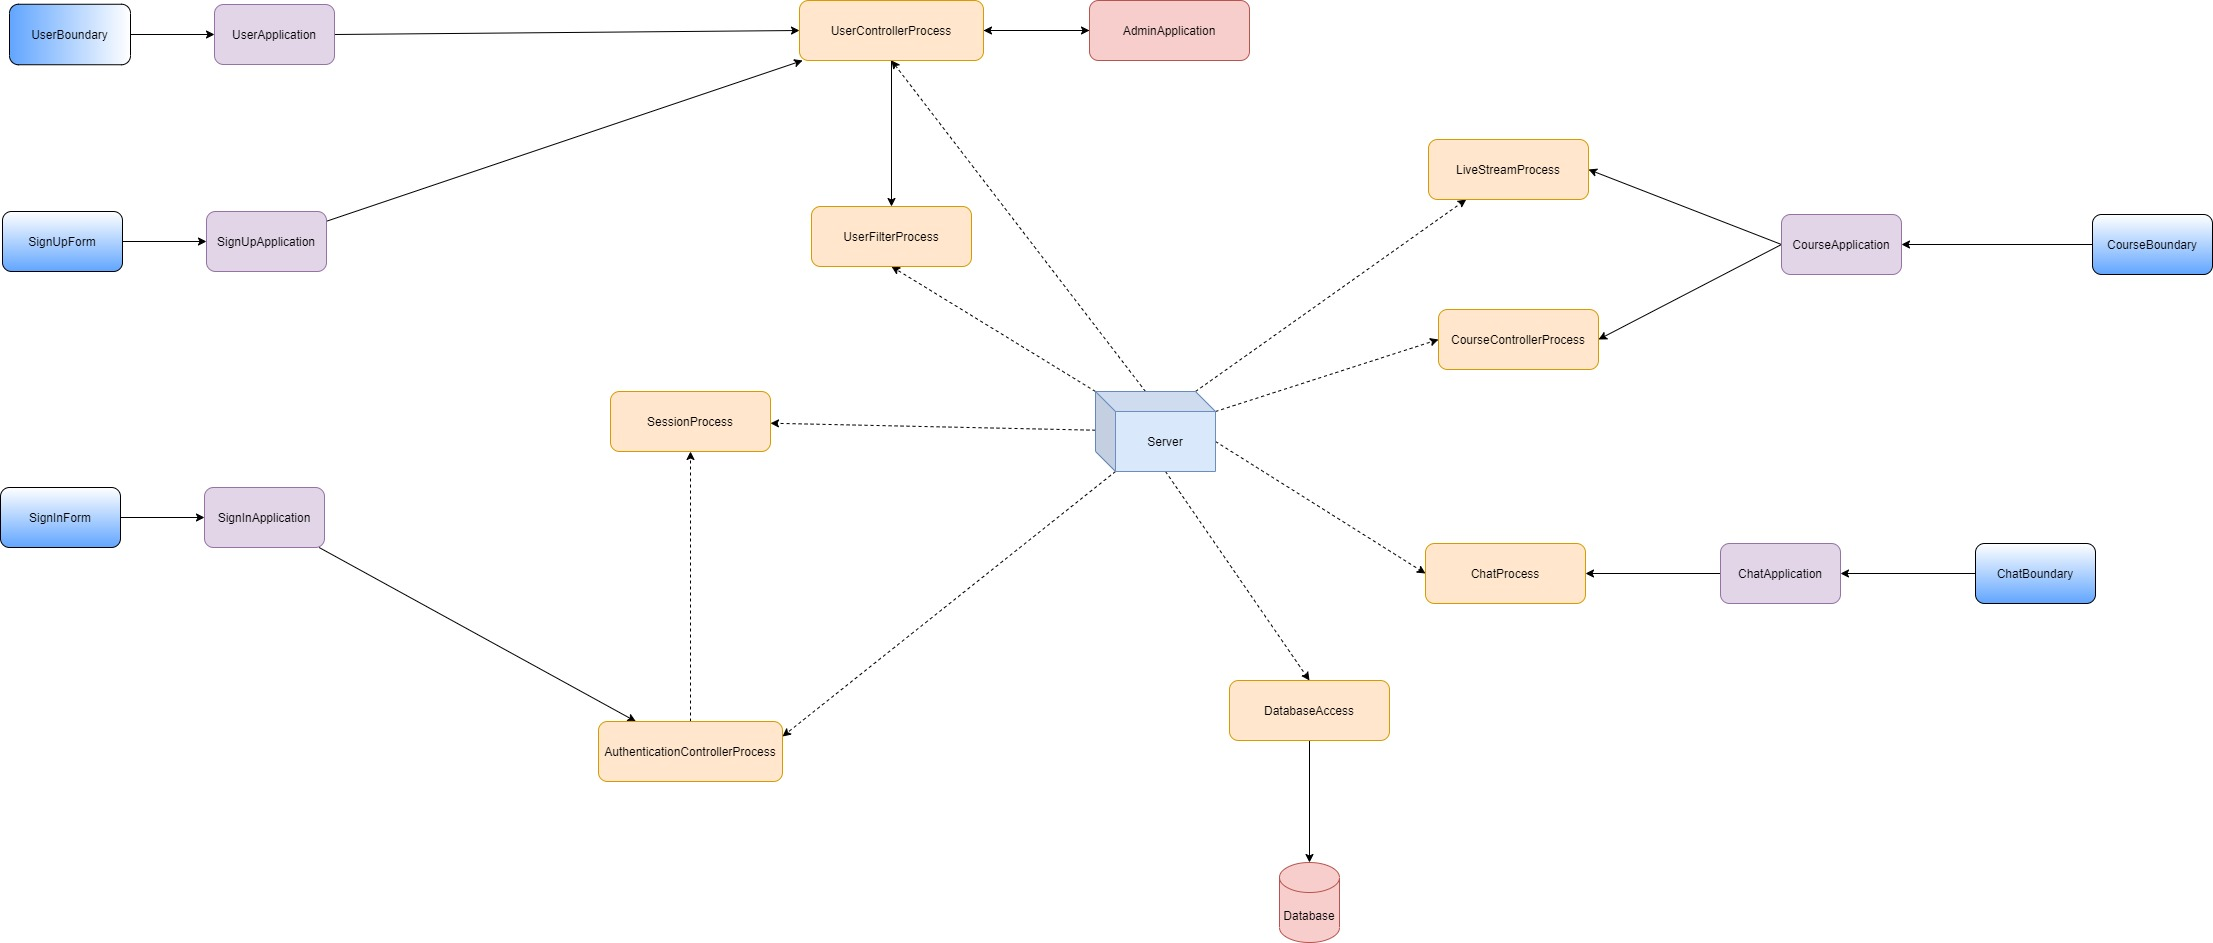
\includegraphics[width=\textwidth]{./images/processview.png}
		\caption{Biểu đồ khung nhìn tiến trình}
	\end{figure}
	\subsection{Mô tả các phần tử tiến trình}
	\begin{description}
		\item[Tiến trình SignUpApplication] Điều khiển các giao diện, biểu mẫu cho người dùng đăng ký vào hệ thống để có thể thao tác, sử dụng các dịch vụ.
		Có một thể hiện của tiến trình này tương ứng với mỗi khách truy cập sử dụng hệ thống.
		\item[Tiến trình SignInApplication] Điều khiển các giao diện, biểu mẫu cho người dùng đăng nhập vào hệ thống để có thể thao tác, sử dụng các dịch vụ.
		Có một thể hiện của tiến trình này tương ứng với mỗi khách đăng nhập hệ thống.
		\item[Tiến trình CourseApplication] Cung cấp giao diện để người dùng thao tác và sử dụng các khóa học cũng như tài liệu khóa học. Có một thể hiện của tiến trình này tương ứng với mỗi khách đăng nhập hệ thống.
		\item[Tiến trình ChatApplication] Cung cấp chức năng chat giữa các người dùng với nhau. Có một thể hiện của tiến trình này tương ứng với mỗi khách đăng nhập hệ thống.
		\item[Tiến trình UserApplication] Cung cấp giao diện, chức năng liên quan đến người dùng trong hệ thống. Có một thể hiện của tiến trình này tương ứng với mỗi khách đăng nhập hệ thống.
		\item[Tiến trình AdminApplication] Điều khiển các giao diện, biểu mẫu dành cho quản trị viên để có thể thao tác, sử dụng các dịch vụ của hệ thống.
		Có một thể hiện của tiến trình này tương ứng với mỗi quản trị viên hệ thống.
		\item[Tiến trình AuthenticationControllerProcess] Quản lý quá trình thực hiện xử lý tạo, xác thực tài khoản người dùng.
		Có một thể hiện của tiến trình này tương ứng mỗi lần khách truy cập đăng ký tài khoản/đăng nhập trên hệ thống.
		\item[Tiến trình UserControllerProcess] Quản lý thông tin người dùng. Có một thể hiện của tiến trình này tương ứng mỗi lần khách truy cập đăng ký tài khoản/đăng nhập trên hệ thống.
		\item[Tiến trình SessionProcess] Quản lý thông tin phiên đăng nhập của từng người dùng. Có một thể hiện duy nhất của tiến trình này trên toàn bộ hệ thống.
		\item[Tiến trình ChatProcess] Xử lý nghiệp vụ nhắn tin giữa các người dùng tương ứng với ChatApplication. Có một thể hiện duy nhất của tiến trình này trên toàn bộ hệ thống.
		\item[Tiến trình LiveStreamProcess] Quản lý, tương tác với module Online livestream để tạo live. Có một thể hiện tương ứng với mỗi lần tạo mới live.
		\item[Tiến trình CourseControllerProcess] Xử lý các yêu cầu và trả về kết quả tương ứng với CourseApplication. Có một thể hiện của tiến trình này tương ứng với mỗi khách đăng nhập hệ thống.
		\item[Tiến trình UserFilterProcess] Quản lý quá trình thực hiện xử lý lọc, tìm kiếm người dùng trên hệ thống. 
		Có một thể hiện của tiến trình này tương ứng với mỗi lần lọc, tìm kiếm người dùng trên hệ thống.
		\item[Tiến trình DatabaseAccess] Quản lý, xử lý các yêu cầu và thao tác liên quan đến database của hệ thống. Có nhiều thể hiện của tiến trình tương ứng với các database của hệ thống kết nối đến.
	\end{description}
\end{document}